%!TEX root = ./main.tex

\section{Online \emph{linear} covering with experts}	\label{sec:covering}

\subsection{Benchmark relaxation for the algorithm}

Our first proposed algorithm solves online linear covering problems by creating linear combinations of the solutions proposed by $K$ experts in an online manner.
Recall that we evaluate the performance of our algorithm with the \texttt{LIN-COMB} benchmark (formalized on \cref{fig:benchmark}), which consists of the best linear combination of the experts' solution at each time step.

Since our \texttt{LIN-COMB} benchmark is a linear combination of the experts' solutions, the equality $ \sum_{k=1}^{K} w_{k}^{t} = 1$ must hold, where $w_{k}^{t} \geq 0$ is the weight assigned to expert $k$ at time~$t$. In the following, we formulate a relaxed version of \texttt{LIN-COMB}, where
$\sum_{k=1}^{K} w_{k}^{t} \geq 1$. The relaxed formulation also enables us to avoid the (online) hard constraint requiring $w_{k}^{t} s_{i,k}^{t} \geq w_{k}^{t-1} s_{i,k}^{t-1}$ to hold. Instead, we introduce a new variable, $y_{i}^{t}$, to represent the increase of $x_{i}^{t}$ compared to $x_{i}^{t-1}$. When $w_{k}^{t} s_{i,k}^{t} < w_{k}^{t-1} s_{i,k}^{t-1}$ during the execution, we set the contribution of $i$ at time $t$ to be 0, and therefore, $y_{i}^{t} = 0$.
The relaxed formulation is visible on Figure~\ref{fig:relaxation}. Due to the relaxation, the optimal solution of the relaxed linear program is a lower bound of our \texttt{LIN-COMB} benchmark. The dual of the relaxation is displayed on Figure~\ref{fig:dual}.


\begin{figure}
	\begin{mdframed}
		\vspace{-10pt}
		\begin{align*}
			&& \min \sum_{t = 1}^{T} \sum_{i=1}^{n} & c_i y_i^t \\
			%
			(\alpha^{t}) \qquad && \sum_{k=1}^{K} w_{k}^{t} & \geq 1  & \forall\ t \\
			%
			(\beta_{i}^{t}) \qquad && \sum_{k=1}^{K} \left(w_{k}^{t} s_{i,k}^{t} - w_{k}^{t-1} s_{i,k}^{t-1} \right) &\leq y_i^t  &\forall\ i,t\\
		%
			&& w_{k}^{t},\ y_{i}^{t} & \ge 0 & \forall\ i,t,k
		\end{align*}
		%\vspace{5pt}
	\end{mdframed}
	\caption{The relaxation of the \texttt{LIN-COMB} benchmark}
	\label{fig:relaxation}
\end{figure}

\begin{figure}
	\begin{mdframed}
	\vspace{-10pt}
		\begin{align*}
			&& \max \sum_{t=1}^{T} & \alpha^{t} \\
		%
			(w_{k}^{t}) \qquad && \alpha^{t} + \sum_{i=1}^{n} s_{i,k}^{t} ( \beta_{i}^{t+1} - \beta_{i}^{t})   &\leq 0  &\forall\ k,t\\
		%
			(y_{i}^{t}) \qquad && \beta_{i}^{t}   &\leq c_{i}  &\forall\ i,t \\
		%
			&& \alpha_{i}^{t},\ \beta_{i}^{t} & \ge 0 & \forall\ i,t
		\end{align*}
	\end{mdframed}
	\caption{The dual of the \texttt{LIN-COMB} benchmark's relaxation}
	\label{fig:dual}
	\vspace{-5pt}
\end{figure}


According to the theorem of weak duality, any feasible solution of the dual program lower bounds any feasible solution of the primal program, and therefore, any feasible dual solution also lower bounds our \texttt{LIN-COMB} benchmark. Following the chain of lower bounds, our approach to design a competitive algorithm is as follows. At every time step $t$, we build solutions for all $x_{i}^{t}$ together with the solutions for the dual problem $(\alpha^{t}, \beta_{i}^{t})$. Then, we bound the cost of the algorithm to that of the dual. It is important to emphasize that the designed solution for every $x_{i}^{t}$ must be feasible to the covering constraints, but it may \emph{not necessarily} be a linear combination of the experts' solutions.

\subsection{Algorithm description} \label{sec:algo}

\paragraph{Preprocessing.}
We recall that by our assumptions, the experts' solutions are always feasible and non-decreasing. At the arrival of the $t^{\text{th}}$ constraint, expert $k$ provides a feasible solution $s_{k}^{t} = (s_{i,k}^{t})_{i=1}^{n}$, such that $s_{i,k}^{t} \ge s_{i,k}^{t'}$ for all $t' \le t$ and all $i$. These assumptions do not exclude the possibility for the experts to provide malicious solutions that instruct the algorithm to use an unnecessarily large amount of resources.
To regardless maintain online solutions, we do \emph{not} expect the experts' solutions to be always tight (a difference compared to the assumptions in \cite{AnandGe22:Online-Algorithms}).
%Either the solutions come from an offline method and guarantee tightness as in \cite{BamasMaggoriSvensson20:primal-dual-method}, or the solutions are constructed online by the experts and do not guarantee tightness.
(In Appendix~\ref{appix-tight-solutions}
we show an example that tight solutions cannot be maintained in an online manner.)

To circumvent the issue of malicious suggestions, we preprocess the experts' solutions at each iteration. During the preprocessing, every solution $s_k^t$ is scaled down to make it as tight as possible on the $t^{\text{th}}$ constraint, while always maintaining $s_{i,k}^{t} \geq s_{i,k}^{t-1}$ for all $i$. Additionally, after the down-scaling, we create an auxiliary solution $\hat{s}_k^t$ that is tight for the $t^{\text{th}}$ constraint. An important highlight: this auxiliary solution is useful for our algorithm and its analysis, but it does \emph{not} directly participate in forming the actual solution. (Our algorithm only sets the weights of the experts and does not change the experts' solutions.) The auxiliary solution $\hat{s}_k^t$ is created with the following procedure.

\break

\paragraph{Preprocessing procedure.} After down-scaling the experts' suggestions, do the following for each expert $k$.
\begin{compactenum}
	\item If $(s_{i,k}^{t})_{i=1}^{n}$ is tight on the $t^{\text{th}}$ constraint, then for every~$i$ set $\hat{s}_{i,k}^{t}~\gets~s_{i,k}^{t}$.
	\item Let $\hat{s}_{i,k}^{t-1}$ be the auxiliary solution of expert $k$ at time $t-1$, meaning that, $\sum_{i=1}^{n} a_{i}^{t-1} \hat{s}_{i,k}^{t-1} = 1$. Given $I := \{i: s_{i,k}^{t} > \hat{s}_{i,k}^{t-1} \cdot \frac{a_{i}^{t-1}}{a_{i}^{t}} \}$, if $i \notin I$
	we set $\hat{s}_{i,k}^{t} \gets s_{i,k}^{t}$, and if $i \in I$, we set $\hat{s}_{i,k}^{t}$ to be some value in $[\hat{s}_{i,k}^{t-1} \cdot \frac{a_{i}^{t-1}}{a_{i}^{t}}, s_{i,k}^{t}]$ such that the solution $\hat{s}_{i,k}^{t}$
	becomes tight on the $t^{\text{th}}$ constraint.
\end{compactenum}

\begin{restatable}{lemma}{preprocessinglemma}
	\label{lem:preprocessing}
	Following the preprocessing procedure, we can always obtain the solutions $\hat{s}_{i,k}^{t}$ such that
	$\hat{s}_{i,k}^{t} \leq s_{i,k}^{t}$ and $\sum_{i=1}^{n} a_{i}^{t} \hat{s}_{i,k}^{t} = 1$.
\end{restatable}
For the proof of \cref{lem:preprocessing} see \cref{appix-proofs}.

\paragraph{Prerequisites.} Our proposed algorithm solves an internal convex program to set the value of $(x_i^t)_{i=1}^n$ at each time step $t$. The convex program's objective uses a shifted entropy function as a convex regularizer. To avoid a possible division by $0$ while solving the convex program, we use a dummy expert. This expert sets initially each variable to some small value, then follows the greedy heuristic and resolves the problem at each arriving constraint. The presence of this dummy expert only changes the competitive ratio from $O(\log(K))$ to $O(\log(K + 1))$, so to simplify the notation, we display all other occurrences of the competitive ratio as $O(\log(K))$. At time $0$ (when no constraints have arrived yet), every expert's suggestion is $0$ for every variable, but the average of the suggestions is $1$.

\paragraph{Algorithm.} The algorithm is visible on \cref{fig:algo1}.

\begin{figure*}
\begin{mdframed}
\paragraph{Algorithm 1.} At the arrival of the $t^{\text{th}}$ constraint,
\begin{compactenum}
	\item solve the following convex program and set $w^t$ to be the obtained optimal solution
%
\begin{align*}
	&& \min_{w} \biggl\{\sum_{i=1}^{n} c_{i}  \biggl[  \biggl(\sum_{k=1}^{K} s_{i,k}^{t} w_{i,k}  + \delta_{i}^{t} \biggr) &
	\ln \left( \frac{\sum_{k=1}^{K} s_{i,k}^{t} w_{i,k}  + \delta_{i}^{t}}{ \sum_{k=1}^{K}  s_{i,k}^{t-1}w_{i,k}^{t-1}  + \delta_{i}^{t-1}}  \right)
	- \sum_{k=1}^{K}  s_{i,k}^{t} w_{i,k} \biggr] \biggr\} \\
	%\end{align*}
	%%
	%\noindent subject to:
	%%
	%\begin{align*}
		(\gamma^{t})  && \sum_{i=1}^{n} a_{i}^{t} \biggl( \sum_{k=1}^{K}  \hat{s}_{i,k}^{t} w_{i,k} \biggr) &\geq 1 \qquad \forall\ t\\
		%
		(\lambda_{i}) && \sum_{k=1}^{K}  w_{i,k} &\geq 1 \qquad \forall\ i\\
		%
		(\mu_{i}^{t}) && \sum_{k=1}^{K} s_{i,k}^{t} w_{i,k} &\geq 0 \qquad \forall\ i,t
	\end{align*}
	%
	where $\delta_{i}^{t} = \frac{1}{K} \sum_{k} s_{i,k}^{t}$.
	%and recall that we set $\rho = \max_{i} \max_{t',t''} \left\{\frac{\sum_{k=1}^{K} s_{i,k}^{t'}}{\sum_{k=1}^{K} s_{i,k}^{t''}} : \sum_{k=1}^{K} s_{i,k}^{t''} > 0 \right\}$.
	We use the auxiliary solution $\hat{s}_{i,k}^{t}$ in the first constraint. For every $i$ where $s_{i,k}^{t} = 0$ for all $k$, the term related to $i$ is not included in the objective function ($w_{i,k} = 0$ for all $k$ beforehand).
	%
	\item For all $i$, if $\sum_{k} w_{i,k}^{t} s_{i,k}^{t} > x_{i}^{t-1}$ then set $x_{i}^{t} \gets \sum_{k} w_{i,k}^{t} s_{i,k}^{t}$;
	otherwise set $x_{i}^{t} \gets x_{i}^{t-1}$.
\end{compactenum}
\end{mdframed}
	\caption{Algorithm 1 for online linear covering problems}
	\label{fig:algo1}
\end{figure*}

\subsection{Performance Analysis}
As $w^{t}$ is the optimal solution of the convex program and ($\gamma^t,\ \lambda_{i},\ \mu_{i}^{t}$) is the optimal solution of its dual, the following Karush-Kuhn-Tucker (KKT) and complementary slackness conditions hold.
First the complementary slackness, primal feasibility, and dual feasibility conditions:
\begin{align*}
   \biggl[ \sum_{i=1}^{n} a_{i}^{t} \biggl( \sum_{k=1}^{K}  \hat{s}_{i,k}^{t} w_{i,k}^{t} \biggr) - 1 \biggr] \gamma^{t} &= 0 \qquad \forall\ t \\
   \biggl[ \sum_{k=1}^{K}  w_{i,k}^{t}  - 1 \biggr] \lambda_{i} &= 0 \qquad \forall\ i, t \\
   \biggl[ \sum_{k=1}^{K}  s_{i,k}^{t} w_{i,k}^{t} \biggr] \mu_{i}^{t} &= 0 \qquad \forall\ i, t \\
   \gamma^{t}, \lambda_{i}, \mu_{i}^{t} &\geq 0 \qquad \forall\ i, t
\end{align*}
And the stationarity condition:
\begin{align*}
	c_{i} s_{i,k}^{t} & \ln \left( \frac{\sum_{k=1}^{K} s_{i,k}^{t} w_{i,k}^{t} + \delta_{i}^{t}}{\sum_{k=1}^{K}  s_{i,k}^{t-1}w_{i,k}^{t-1}  + \delta_{i}^{t-1}} \right) & \\
    	& - a_{i}^{t} \hat{s}_{i,k}^{t} \gamma^{t} - \lambda_{i} - s_{i,k}^{t} \mu_{i}^{t} &= 0	\qquad \forall\ i,k,t
\end{align*}

Moreover, if $\sum_{k} w_{i,k}^{t} s_{i,k}^{t} > 0$, meaning that $\mu_{i}^{t} = 0$, then
\begin{align}	\label{eq:KKT1}
   c_{i} s_{i,k}^{t} \ln \left( \cdots \right)
    	 - a_{i}^{t} \hat{s}_{i,k}^{t} \gamma^{t} - \lambda_{i}  = 0
\end{align}
where the logarithm contains the same fraction as above.

\paragraph{Dual variables and feasibility.} We set the dual variables of the linear program relaxation of our \texttt{LIN-COMB} benchmark based on the dual variables of the convex program used inside the algorithm. We recall that the dual formulation is visible on \cref{fig:dual}.
%
\begin{align*}
    \alpha^{t} &= \frac{1}{\ln(K\rho)}  \biggl( \gamma^{t} + \sum_{i=1}^{n} \lambda_{i} \biggr), \\
    \beta_{i}^{t} &= \frac{1}{\ln(K\rho)} c_i \ln \left(\frac{ (1 + 1/K) \cdot \max_{t'} \sum_{k=1}^{K} s_{i,k}^{t'}}{\sum_{k=1}^{K}  s_{i,k}^{t-1} w_{i,k}^{t-1} + \delta_{i}^{t-1}}\right)
\end{align*}
%
where we recall that
\[
	\rho = \max_{i, t',t''} \left\{\frac{\sum_{k=1}^{K} s_{i,k}^{t'}}{\sum_{k=1}^{K} s_{i,k}^{t''}} : \sum_{k=1}^{K} s_{i,k}^{t''} > 0 \right\}.
\]

\begin{restatable}{lemma}{coveringfeasibility}
	\label{lem:covering-feasibility}
	The $x_{i}^{t}$ solutions set by the algorithm for the original covering problem and the dual variables $(\alpha^{t}, \beta_{i}^{t})$ of the \texttt{LIN-COMB} benchmark's linear program relaxation are feasible.
\end{restatable}
For the proof of \cref{lem:covering-feasibility} see \cref{appix-proofs}.

\begin{theorem} \label{covering-theorem}
Algorithm 1 is $O(\ln(K \rho))$-competitive with the \texttt{LIN-COMB} benchmark.
\end{theorem}
%
\begin{proof} \cref{lem:covering-feasibility} proved that our algorithm creates feasible solutions for the dual problem of the \texttt{LIN-COMB} benchmark's relaxation and for the original covering problem. We show that the algorithm's solution increases the primal objective value of the original covering problem by at most $O(\ln(K \rho))$ times the value of the relaxation's dual solution, which serves as the lower bound on the \texttt{LIN-COMB} benchmark (the best linear combination of the experts' solutions).

\begin{align}
	 \sum_{i=1}^{n} &c_{i} (x_{i}^{t} - x_{i}^{t-1}) & \notag \\
		&= \sum_{i: x_{i}^{t} > x_{i}^{t-1}} c_{i}(x_{i}^{t} - x_{i}^{t-1})  \notag \\
		%
		&\leq \sum_{i: x_{i}^{t} > x_{i}^{t-1}} c_{i}(x_{i}^{t} + \delta_{i}^{t}) \ln \left(\frac{x_{i}^{t} + \delta_{i}^{t}}{x_{i}^{t-1} + \delta_{i}^{t}}\right)
\end{align}

\begin{align}
    \leq \sum_{i: x_{i}^{t} > x_{i}^{t-1}} c_{i} & (x_{i}^{t} + \delta_{i}^{t}) \ln \left(\frac{x_{i}^{t} + \delta_{i}^{t}}{x_{i}^{t-1} + \delta_{i}^{t-1}}\right) \\
    %
    = \sum_{i: x_{i}^{t} > x_{i}^{t-1}} c_{i} & \left[ \left(\sum_{k=1}^{K}  s_{i,k}^{t} w_{i,k}^{t} + \frac{1}{K} \sum_{k=1}^{K} s_{i,k}^{t} \right)  \notag  \right. \\
		& \left. \ \ \ \ \ln \left(\frac{ \sum_{k=1}^{K}  s_{i,k}^{t} w_{i,k}^{t} + \delta_{i}^{t}}{x_{i}^{t-1} + \delta_{i}^{t-1}}  \right) \right] \\
    %
    \leq \sum_{i: x_{i}^{t} > x_{i}^{t-1}} c_{i} & \left[ \left(\sum_{k=1}^{K}  s_{i,k}^{t} w_{i,k}^{t} + \frac{1}{K} \sum_{k=1}^{K} s_{i,k}^{t} \right) \notag \right. \\
            & \left. \ \ \ \ \ln \left(\frac{ \sum_{k=1}^{K} s_{i,k}^{t} w_{i,k}^{t} + \delta_{i}^{t}}{\sum_{k=1}^{K}  s_{i,k}^{t-1} w_{i,k}^{t-1} + \delta_{i}^{t-1}}  \right) \right]\\
    %
    = \sum_{i: x_{i}^{t} > x_{i}^{t-1}} \ \ \ \ & \sum_{k=1}^{K} (w_{i,k}^{t} + 1/K) c_{i} s_{i,k}^{t} \notag \\
            & \ \ \ \ \ln \left(\frac{ \sum_{k=1}^{K} s_{i,k}^{t} w_{i,k}^{t}  + \delta_{i}^{t}}{\sum_{k=1}^{K} s_{i,k}^{t-1} w_{i,k}^{t-1}  + \delta_{i}^{t-1}}  \right) \notag \\
    %
    = \sum_{i: x_{i}^{t} > x_{i}^{t-1}} \ \ \ \ & \sum_{k=1}^{K} (w_{i,k}^{t} + 1/K) \biggl( a_{i}^{t} \hat{s}_{i,k}^{t} \gamma^t + \lambda_{i} \biggr) \\
    %
    \leq \ \ \ \ \sum_{i=1}^{n} \ \ \ \ \ \ \ \ & \sum_{k=1}^{K} (w_{i,k}^{t} + 1/K) \biggl( a_{i}^{t} \hat{s}_{i,k}^{t} \gamma^t + \lambda_{i} \biggr) \notag \\
    %
    = 2 \gamma^{t} + 2 \sum_{i=1}^{n} & \lambda_{i} = 2\ln(K \rho) \alpha^{t}
\end{align}

The justification for the previous transformations:
\begin{compactenum}[(1)]
	\setcounter{enumi}{1}
	\item follows from the inequality $a - b \leq a \ln(a/b)$ for all $0 < b \leq a$;
	\item holds since $\delta_{i}^{t} \geq \delta_{i}^{t-1}$ (because $s_{i,k}^{t} \geq s_{i,k}^{t-1}$ for all $i,k,t$);
	\item is valid because $x_{i}^{t} > x_{i}^{t-1}$, so $x_{i}^{t} = \sum_{k}  s_{i,k}^{t} w_{i,k}^{t}$;
	\item by the algorithm's design: $x_{i}^{t-1} \geq \sum_{k}  s_{i,k}^{t-1} w_{i,k}^{t-1}$;
	\setcounter{enumi}{5}
	\item since $x_{i}^{t} > x_{i}^{t-1} \geq 0$
	(so $\sum_{k}  s_{i,k}^{t} w_{i,k}^{t} = x_{i}^{t} > 0$), the stationarity KKT condition (\ref{eq:KKT1}) applies;
	\item is true due to the complementary slackness conditions
		and because $\sum_{i} a_{i}^{t}  \hat{s}_{i,k}^{t} = 1$.
\end{compactenum}
\end{proof}

\begin{corollary} \label{corollary}
	For $0$-$1$ optimization problems in which the experts provide integer (deterministic or randomized) solutions,
	our algorithm is $O(\ln (K))$-competitive with the \texttt{LIN-COMB} benchmark.
	Further, there exists an algorithm whose performance is $O(\ln (K))$-competitive with the \texttt{LIN-COMB}
	benchmark and is up to a constant factor far from the best guarantee in the worst-case benchmark.
\end{corollary}
%
\begin{proof}

	\begin{figure}[!ht]
		\centering
		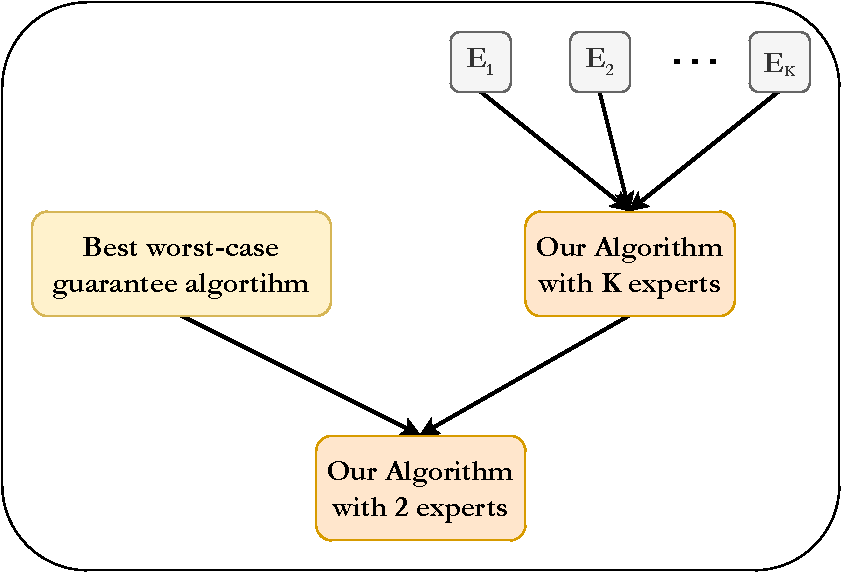
\includegraphics[width=0.4\textwidth]{../paper/Img/algo_structure.pdf}
		\caption{Structural overview of the algorithm's components. $E_1,\ E_2, \dots\ E_K$ correspond to the experts of the online problem. On the second layer, we integrate the best standard online algorithm with our algorithm. }
		\label{fig:algo-layers}
	\end{figure}

	\noindent If the value of $s_{i,k}^{t}$ is in $\{0,1\}$ for every $i,k,t$, then
	\[
	\rho = \max_{i} \max_{t',t''} \left\{\frac{\sum_{k=1}^{K} s_{i,k}^{t'}}{\sum_{k=1}^{K} s_{i,k}^{t''}} : \sum_{k=1}^{K} s_{i,k}^{t''} > 0 \right\}
	\leq \frac{K}{1}
	\]
	Therefore, the competitive ratio of the our algorithm with the \texttt{LIN-COMB} benchmark is $O(\log (K \rho)) = O(\log (K^2))$.

 	To obtain an algorithm that is competitive with both the \texttt{LIN-COMB} and the worst-case benchmarks, we proceed as follows (\cref{fig:algo-layers} serves as an illustration).
	We first apply the main algorithm on the $K$ experts' integer predictions to obtain an online algorithm, named $A$.
	Algorithm $A$ is $O(\ln (K))$-competitive with the \texttt{LIN-COMB} benchmark. Let $B$ be the algorithm with the best worst-case guarantee.
	We then apply the main algorithm one more time on two algorithms, $A$ and $B$. The final algorithm is $O(\ln (2))$-competitive with both $A$ and $B$.
	In other words, its performance is $O(\ln (K))$-competitive with the \texttt{LIN-COMB} benchmark and is up to a constant factor worse than the best guarantee in the worst-case benchmark.
\end{proof}

\section{Online \emph{convex} covering with experts}

Linear programs are suitable to represent many optimization problems, and they are an essential tool in optimization. However, some practically relevant problems (for example, makespan minimization and congestion management) have non-linear objective functions. We take a step further towards a general framework which can handle such problems as well, and propose an algorithm with multiple experts for $0$-$1$ optimization problems with convex objectives and linear constraints. Due to the page limitations, we only detail this setting in \cref{sec:convex}.
